\documentclass[12pt,twocolumn]{article}
\usepackage[T1]{fontenc}
\usepackage{graphicx}
\usepackage{tabularx}
\usepackage{amsmath,amsthm,amssymb}
%\usepackage{esvect}
\usepackage[left=1cm,right=1cm,top=2cm,bottom=2cm]{geometry}
%\renewcommand*{\familydefault}{\sfdefault}
\title{\vspace{-2.5em}Diffusion in 2 Dimensions}
\author{Christopher Pattison}
\date{}
\begin{document}
\maketitle

\begin{figure}
\label{fig:solution}
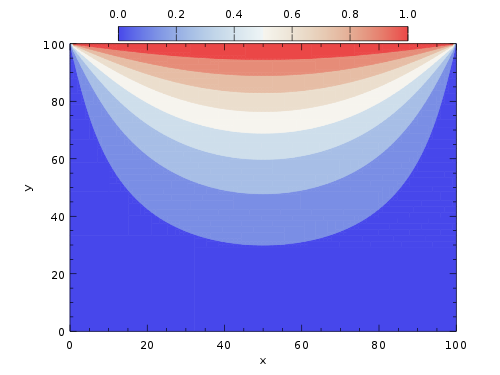
\includegraphics[width=\columnwidth]{plot/solution.png}
\footnotesize{\caption{Solution on a 100x100 cell domain}}
\end{figure}
\section*{Derivation}
The Poisson equation was descretized using the finite volume method.
\begin{equation}\int_V (\nabla \cdot k \nabla T - q )dV = 0\end{equation}
As usual, a residual is defined and then integrated over the control volume.
Using the divergence theorem and the assumption that $q$ and $k$ are invariant, this can be restated as equation \eqref{eq:fvmdiv}.
\begin{equation}\label{eq:fvmdiv}\sum\limits_N \vec{S}_N\cdot k\nabla T - qV = 0\end{equation}
The last step is to approximate the gradient $\nabla T$ which is taken as equation \eqref{eq:gradapprox} where $\vec{x}$ is the node position and $S$ is the area of the cell face.
\begin{equation}\label{eq:gradapprox}\nabla T_n \approx \frac{T_N - T_P}{|\vec{x}_N-\vec{x}_P|}S\end{equation}
On a structured quadrilateral grid with no skewed cells, $\vec{x}$ can be treated as a scalar. If the grid is uniform, then $|\vec{x}_N - \vec{x}_P| = S$.
The coefficients are then simply
\begin{equation}a_N=a_S=a_E=a_W=k\end{equation}
\begin{equation}a_P = -\sum\limits_N a_N \end{equation}

\section*{Solvers}
The resulting coefficient matrix consists of a tridiagonal portion and two bands. Since the coefficient matrix is no longer tridiagonal, a direct solver becomes extremely expensive.

\subsection*{Gauss-Seidel}
Gauss-Seidel is a good choice of solver since the simplicity means that no copy operations have to be carried out. 
Moreover, there is no inconvenience to leaving the coefficient matrix in a form that allows easy handling of the solution vector.
\paragraph{}
In this solver, T was a 2-dimensional array with indicies corresponding to the location of the node in the domain. 
Conveniently, node positions as well as cell neighbors do not have to be stored.
\begin{equation}T_{i,j} =( T_{i+1,j}a_E \dots T_{i,j-1}a_S - b_{i,j})/a_P\end{equation}
\subsection*{Line Solver}
Since TDMA cannot be used on a banded matrix, one option is to hold some of the bands constant which allows the matrix to be put in tridiagonal form.
While this should result in faster dissemination of the boundary conditions into the domain, a coefficient matrix must be explicitly formed. 
This tradeoff can result in poor performance.
\subsection*{Hybrid Solver}
Two hybrid solvers were created that use the line solver before Gauss-Seidel based on the theory that the line solver is 
much quicker than Gauss-Seidel to provide a rough solution.
\paragraph{}A single iteration of Hybrid 1 uses two iterations of the line solver sweeping through the X and Y directions respectively following up with 16 iterations of Gauss-Seidel.
\paragraph{}Hybrid 2 uses the line solver to approximate a solution with a high residual, it then iterates with Gauss-Seidel until convergence.

\begin{figure}
\label{fig:solution}
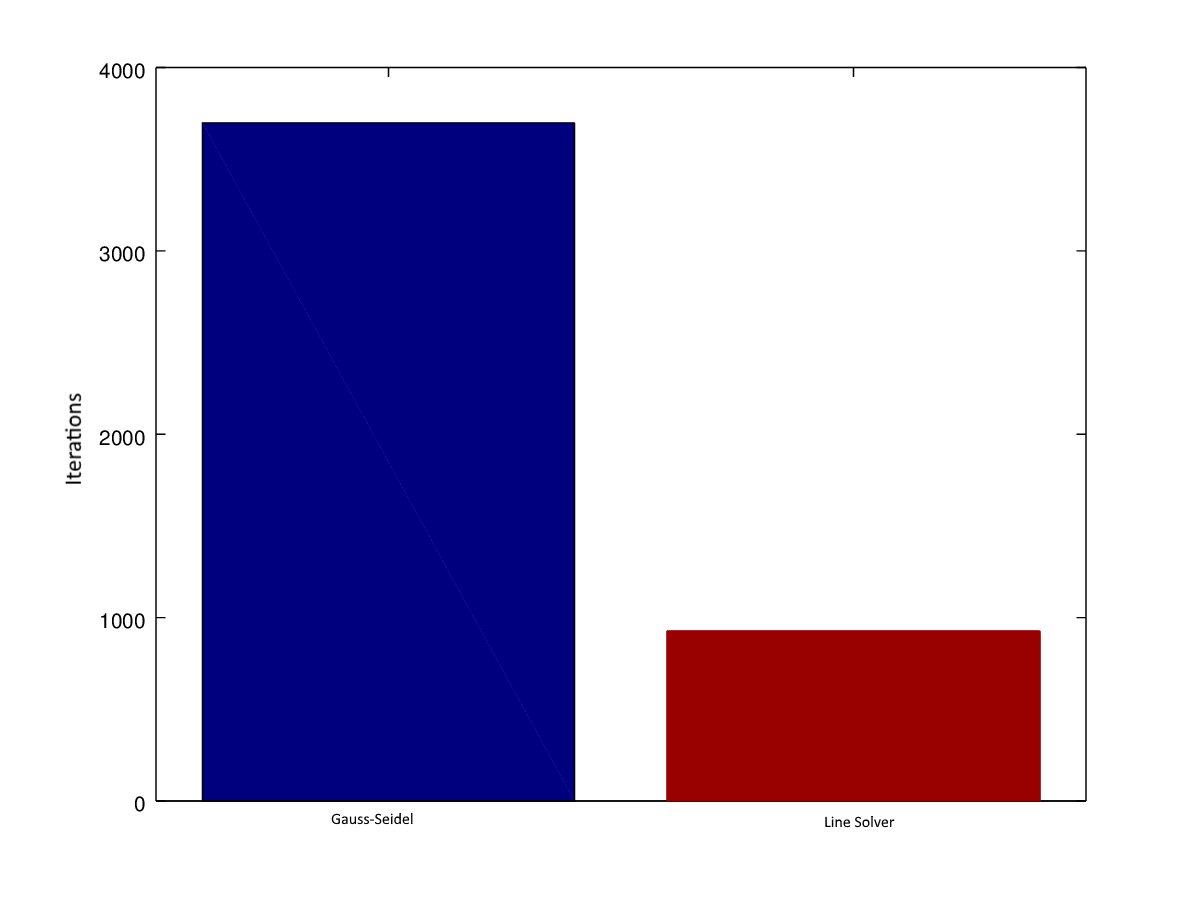
\includegraphics[width=\columnwidth]{plot/iterations.png}
\footnotesize{\caption{Iteration Comparison}}
\end{figure}

\section*{Performance}
The comparisons were made on a 100x100 uniform grid solving for the solution shown in figure 1. The required residual for convergence was $10^{-6}$.
\paragraph{}
While the line solver used fewer iterations to obtain a solution, the computational cost per iteration was higher, resulting in a longer time to completion.
\paragraph{}
Since the hybrid solvers use many sub-iterations, it is difficult to make a meaningful comparison on the basis of iteration.
However, the wall time can be compared quite easily.
\paragraph{} It is notable that Hybrid 2 performed the best as it supplies a rough initial guess obtained with the line solver to Gauss-Seidel,
supporting the basis on which the hybrid solvers were implemented.
\begin{figure}
\label{fig:solution}
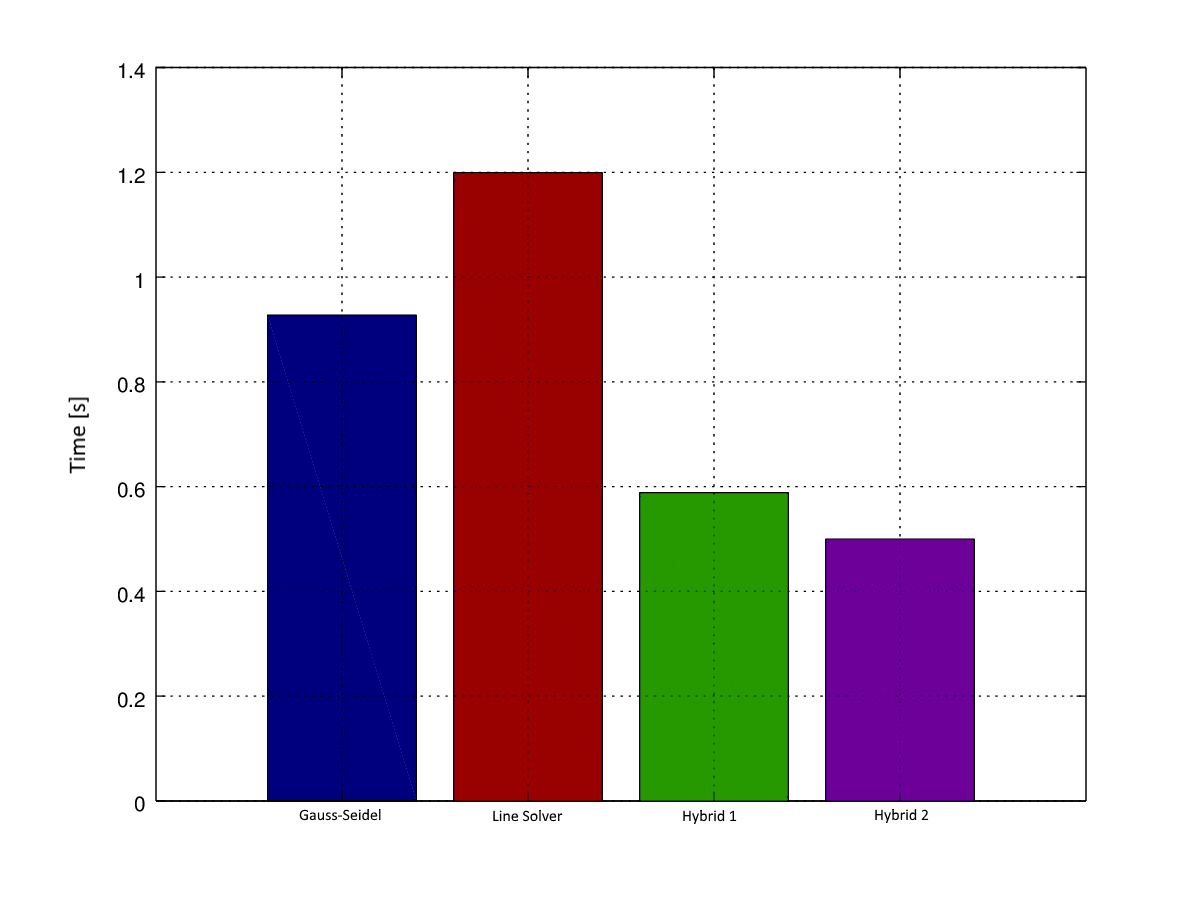
\includegraphics[width=\columnwidth]{plot/walltime.png}
\footnotesize{\caption{Wall Time Comparison}}
\end{figure}
\end{document}

